\chapter{Background}
\label{chap:background}
% ================================================================
% INTRODUCTION TO BCI
\section{Introduction to BCI}
The communication within the human body requires muscles and  peripheral nerves. The start of the process happens with  the user's intent which triggers a complex process where specific brain areas are triggered, and hence the peripheral nerves system sends the signals to the corresponding muscles, which performs the intended action. Efferent means sending signals from the peripheral nervous system to the muscles. However, Afferent describes the other way around. \cite{inbook1}\par
% ----------------------------------------------------------------
A \ac{bci} offers an alternative way to natural control and communication by bypassing the normal efferent pathways. \ac{bci} directly measures the brain waves corresponding to the user intent then translates it into signals which gets sent to the \ac{bci} applications. These translations include enhancement, noise removal, signal processing and pattern detection (classification). \cite{inbook1}\par
% ----------------------------------------------------------------
\ac{bci}, \ac{bmi} and \ac{dbi} almost refers to the same thing which refer to intercepting (recording) brain waves. However, Neuroprosthesis is more general as it refers to receiving and sending signals from and to the brain. Figure \ref{fig:neuroprostheses} shows examples of neuroprostheses which shows that \ac{bci} is a category of neuroprostheses.\par
\begin{figure}
    \centering
    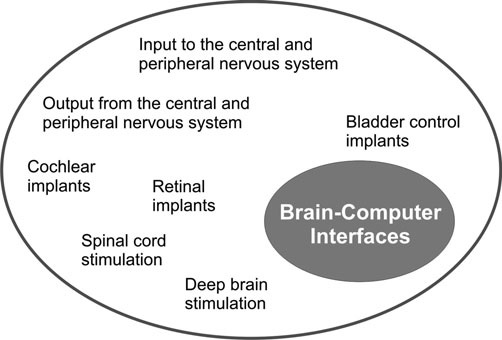
\includegraphics[width=\figureWidth]{images/background/neuroprostheses.jpg}
    \caption{Examples of neuroprostheses and its relation to \ac{bci} \cite{inbook1}}
    \label{fig:neuroprostheses}
\end{figure}
% ----------------------------------------------------------------
\subsection{Processes of Operation}
BCI goes through three main procedures, measuring the brain activity, processing it and controlling the intercepted signals.\par
% ----------------------------------------------------------------
\subsubsection{Measuring Brain Activity}
Brain activity produces magnetic and electrical waves. That’s why, sensors or electrodes are used to measure these changes at different areas and times. Brain activities can be recorded through sensors (non-surgical solution) or electrodes (surgical solutions). For the non-surgical solution, sensors are used to measure the electrical activity from the scalp and this solution is called \ac{eeg} (Figure \ref{fig:eeg}). They are relatively easy to deal with however they don’t provide accurate measures due to external interference and are susceptible to limitations in frequency range. In order to get consistent recording, sensors are spread on the scalp through system called 10 - 20 (Figure \ref{fig:10-20-system}). 10 - 20 refers to how sensors are spread 10 - 20 - 20 - 20 - 20 - 10 percent. The 6 regions are named according to their position: Fp - pre-frontal, F - frontal, C - central, P - parietal, O - occipital, T - temporal.\par
\begin{figure}
    \centering
    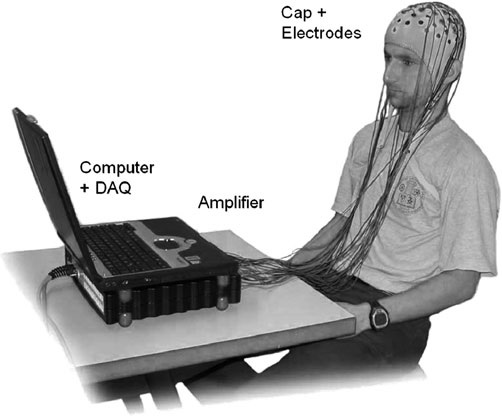
\includegraphics[width=\figureWidth]{images/background/eeg.jpg}
    \caption{\ac{eeg} based \ac{bci} \cite{inbook1}}
    \label{fig:eeg}
\end{figure}
\begin{figure}
    \centering
    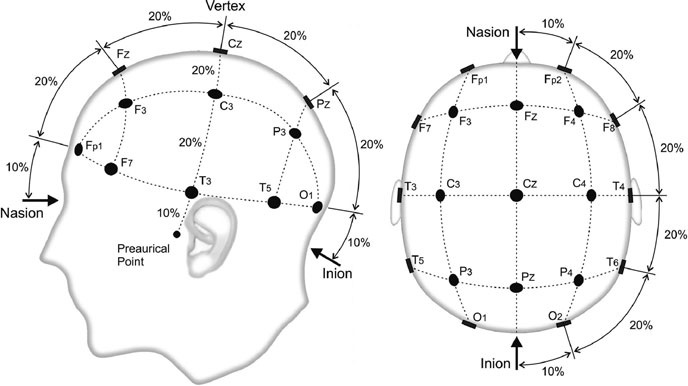
\includegraphics[width=\figureWidth]{images/background/10_20_system.jpg}
    \caption{International standard of representing 10 - 20 system that shows how electrodes are spread on the scalp \cite{inbook1}}
    \label{fig:10-20-system}
\end{figure}
% ----------------------------------------------------------------
On the other hand, the surgical solution need to open the skull through surgical procedures and plant the electrodes. When the electrodes are planted on the surface of the cortex, it’s called \ac{ecog}.\par
% ----------------------------------------------------------------
And another solution called \ac{icr}, which plants the electrodes in the inner parts of the brain. Although the surgical solutions provide higher accuracy and frequency range compared to the non-surgical solution they have serious drawbacks such as they need surgery, finance and can have ethical problems. Difference between each solution is shown in Figure \ref{fig:brain-waves-detection}.\par
\begin{figure}
    \centering
    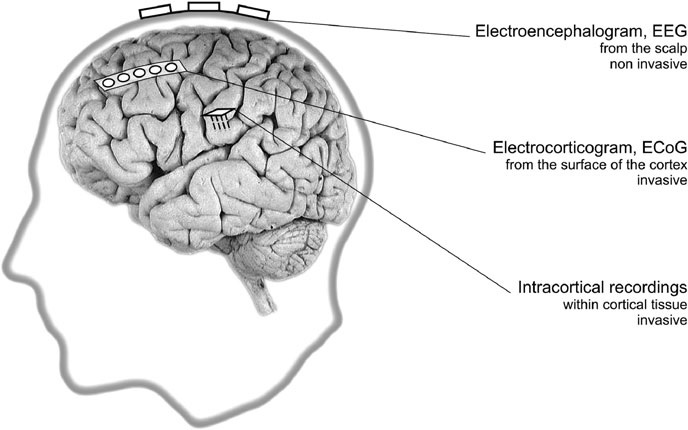
\includegraphics[width=\figureWidth]{images/background/brain-waves-detection.jpg}
    \caption{The surgical and non-surgical solutions of brain waves' detection \cite{inbook1}}
    \label{fig:brain-waves-detection}
\end{figure}
% ----------------------------------------------------------------
\subsection{Brain Patterns}
Because measuring brain activity is not enough, some mental strategies are used to trigger the required tasks. The most used mental strategies are selective attention and motor imagery. Since only selective attention is needed in this project, motor imagery will not be introduced.\par
% ----------------------------------------------------------------
\subsubsection{Selective Attention}
\ac{bci} based on selective attention has to depend on external stimuli (event), either visual or auditory. In \ac{bci} application, in order for the user to select certain command, the user has to focus (select) their attention on a certain item on the screen to execute that command.\par
% ----------------------------------------------------------------
\ac{p300} based \ac{bci}, the main component behind this project, relies on visual stimuli to execute different tasks. As described in Chapter \ref{chap:introduction}, \ac{p300} is an oddball paradigm that requires two kind of events, frequent and infrequent event. However, infrequent events must be by surprise to show the most effect (Figure \ref{fig:p300-signal}).\par
\begin{figure}[!ht]
    \centering
    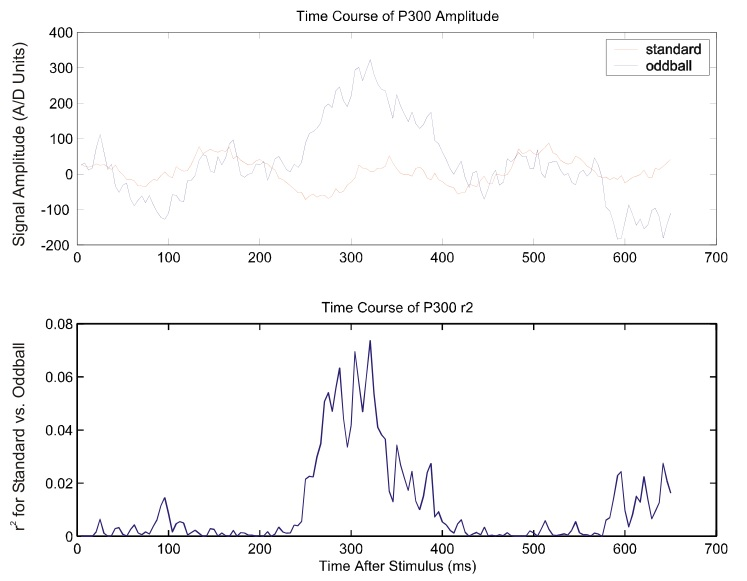
\includegraphics[width=\figureWidth]{images/background/p300_signal.jpg}
    \caption{\ac{p300} Signal: Representation of an oddball paradigm \cite{article1}.}
    \label{fig:p300-signal}
\end{figure}
% ----------------------------------------------------------------
\ac{ssvep} based \ac{bci} is similar to \ac{p300} as it depends on visual stimuli. \ac{ssvep} requires the screen to flicker with frequencies 6 - 30 Hz to execute different commands. Focusing one's attention on a certain area with certain flickering frequency, then identifying that frequency to execute the wanted task.
% ----------------------------------------------------------------
\clearpage
% ================================================================